\section{[Complete] The Partner Controller}

VEX Robotics once sold a "partner controller" that allowed two controllers to control a robot. However, as of 2021, they are discontinued. This aims to fix that for good.

\begin{figure}[h]
    \centering
    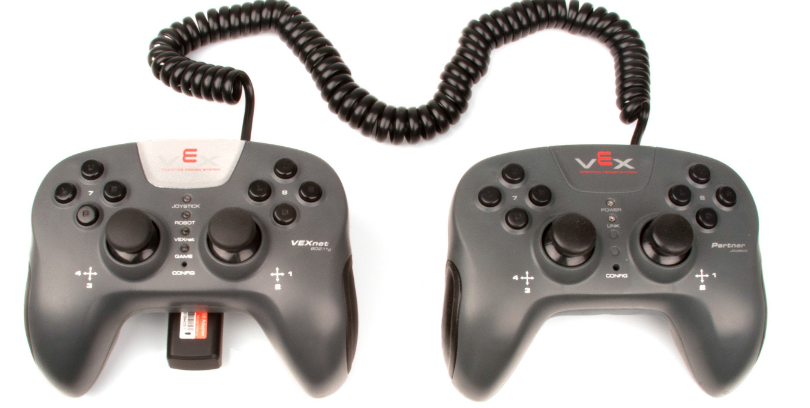
\includegraphics[width=\textwidth,height=10cm,keepaspectratio=true]{PartnerExample}
    \caption{
        A discontinued partner controller (right) being connected to a regular VEXnet controller (left).
    }
\end{figure}

Two posts peaked my interest when researching this. One \cite{PartnerCite2}, stating that the cable needed to connect these controllers together is simply an old-school 4-conductor phone cable, and the second \cite{PartnerCite1}, stating that regular VEXnet controllers have firmware that allows them to act as partner controllers.

\begin{figure}[h]
    \centering
    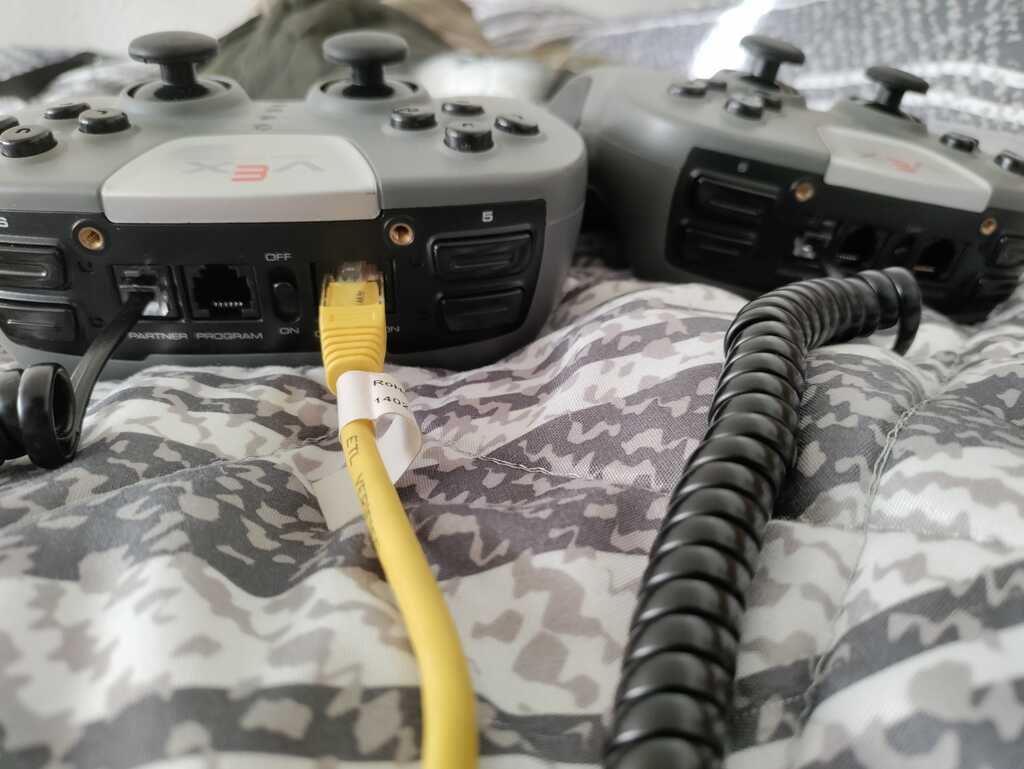
\includegraphics[width=\textwidth,height=10cm,keepaspectratio=true]{Partner1}
    \caption{
        Picture of an ethernet port and telephone port on the VEXnet controller. The telephone cable is used to connect a partner controller, and the ethernet port is used to switch between autonomous and competition mode using a VEX competition switch \cite{VEXCompSwitch}. (You can also make a competition switch yourself \cite{VEXDIYCompSwitch}) The unused port in the middle is a proprietary port used for wireless programming via a VEX programming kit \cite{VEXProgrammingKit}.
    }
\end{figure}


\begin{figure}[h]
    \centering
    \includegraphics[width=\textwidth,height=10cm,keepaspectratio=true]{Partner2}
    \caption{
        Picture of a secondary controller being used to control the robot via a telephone cable connecting both controllers together.
    }
\end{figure}

Instinctively, I tried to use an ethernet cable into the port. After all, they had a very similar designs to a telephone cable. Surprisingly, I accidentally found the cable used for a VEX competition switch \cite{VEXCompSwitch}, which is used to switch between autonomous and manual control during competition. Eventually, I went around to buying a coiled telephone cable, connected the controllers, and successfully made a program that allowed both controllers to be used on the same robot.
